\documentclass[12pt,a4paper,titlepage,twoside]{report}
\usepackage[utf8]{inputenc}
\usepackage[french]{babel}
\usepackage[T1]{fontenc}
\usepackage{amsmath}
\usepackage{amsfonts}
\usepackage{amssymb}
\usepackage{graphicx}
\usepackage{url}
\usepackage[usenames,dvipsnames]{xcolor}
\usepackage[colorlinks=false,urlbordercolor=white,linkbordercolor=white]{hyperref}
\usepackage[left=2cm,right=2cm,top=2cm,bottom=2cm]{geometry}
\usepackage{fancyhdr}
\usepackage{lmodern}
\usepackage{listings}
\pagestyle{fancy}
\usepackage{titlesec}
\usepackage[abs]{overpic}

% Definition des couleurs
\definecolor{titreColor}{RGB}{0,58,128}  % Marine
\definecolor{stitreColor}{RGB}{0,158,224}  % Ocean
\definecolor{auteurColor}{RGB}{0,58,128}     % Marine
\definecolor{texteColor}{RGB}{164,196,0}     % Prairie

% Definition des chapitres
\titleformat{\chapter}[display]
{\normalfont\Large\filcenter\sffamily}
{\titlerule[1pt]%
 \vspace{1pt}%
 \titlerule
 \vspace{1pc}%
 \Large\color{titreColor}{\MakeUppercase{\chaptertitlename} \thechapter}}
{1pc}
{\titlerule
 \vspace{1pc}%
 \Huge}

\titleformat{\section}
{\color{titreColor}\normalfont\Large\bfseries\sffamily}
{\color{titreColor}\thesection}{1em}{}

\titleformat{\subsection}
{\color{stitreColor}\bfseries\sffamily}
{\color{stitreColor}\thesubsection}{1em}{}

%Données de titre et d'auteur pour la page de garde
\newcommand{\titre}{Développement d'une application web}
\newcommand{\sousTitre}{Stage de fin d'étude en DUT informatique}
\newcommand{\auteur}{Maxime Boisse}
\newcommand{\dateModif}{\today}

\begin{document}
%Supprime les veuves et orphelines
\widowpenalty=10000
\clubpenalty=10000
\raggedbottom 

% Integre la page de garde
%\input{title.tex}
%\setcounter{page}{0}
\thispagestyle{empty}
\vspace*{7cm}
\setlength\unitlength{1mm}
% Logo de titre
\begin{overpic}[width=9.44cm,height=9.57cm,keepaspectratio]{logo_fond.png}
% Titre du document
\put(30,50){
\begin{minipage}{0.7\linewidth}
\Huge\flushleft \color{titreColor}{\bfseries\sffamily\titre{}}\\
% sous-titre du document
\color{stitreColor}{\Large \bfseries\sffamily\sousTitre{}}
\end{minipage}
}
\end{overpic}

%  date et auteur
% creation de l'espace a gauche
\vspace*{1cm}
\begin{minipage}{0.5\linewidth}
\hfill
\end{minipage}
% positionnement
\begin{minipage}{0.5\linewidth}\flushleft{
% Date
\textcolor{auteurColor}{\Large\sffamily\dateModif{}}\\
\vspace*{0.1cm}
% Auteur
\textcolor{auteurColor}{\Large\sffamily\auteur{}}\\
\vspace{0.5cm}
% Adresse
\textcolor{texteColor}{\sffamily\textbf{IRSTEA} - Centre de Bordeaux\\
50, avenue de Verdun, Gazinet\\
33612 CESTAS Cedex }
}
\end{minipage}
% Ligne de logos
\begin{minipage}{\linewidth}
% Logo IRSTEA
\vspace{1.3cm}
\hspace{-1.4cm}
\includegraphics[width=3.06cm,height=9.57cm,keepaspectratio]{logo_irstea}%
% logos complémentaires
\vspace{-1cm}
\hspace{12cm}
\includegraphics[width=3cm,height=3cm,keepaspectratio]
{pictures/logo_couleur.jpg}%
\end{minipage}
% Définition des entêtes
\fancyhead{}
\fancyhead[CO]{\leftmark\sffamily}
\fancyhead[CE]{ \sffamily\titre{}}
\fancyfoot[CO]{\sffamily\thepage}
\fancyfoot[CE]{\sffamily\thepage}
% Redéfinition de \cleardoublepage pour créer une page vide
\makeatletter
\def\cleardoublepage{\clearpage\if@twoside \ifodd\c@page\else
  \hbox{}
  \vspace*{\fill}

  \vspace{\fill}
  \thispagestyle{empty}
  \newpage
  \if@twocolumn\hbox{}\newpage\fi\fi\fi}
\makeatother
\lstset{ breaklines=true}

% \cleardoublepage permet de générer une page vide 
% si le chapitre ne commence pas sur la page de droite
\cleardoublepage
\LARGE{Résumé}\normalsize\newline
 	
Le centre de recherche de Cestas a axé ses recherches autour de deux grands domaines : \textbf{la gestion de l'eau et du fonctionnement des milieux aquatiques} et \textbf{l'interface entre eau et gestion des territoires.} 
Au sein de cet établissement, le service informatique supervise le parc informatique et développe différentes applications utilisées pour la recherche. 
L'objectif de ce stage peut se diviser en deux grandes tâches : une partie conception et analyse où l'on étudie le problème et les besoins exprimés. Une seconde partie développement, c'est à dire la création de l'application, en réponse au cahier des charges.
Au cours de ces dix semaines, de nombreux outils et structures ont été utilisés et c'est à travers ce rapport que l'on va les présenter plus en détails. Nous allons aussi voir une présentation d'Irstea et du travail effectué pendant le stage. \newline

\LARGE{Abstract}\normalsize\newline

The research center of Cestas focused its analysis around two main domains :  \textbf{the water management and the fonctionning of the aquatic environments} and \textbf{the interface between water and territories management.} 
Within this institution, the IT service oversee the computer park and develop different applications used by the reserchers.
The goal of this placement can be split into two main parts. On the one hand, a conception and analysis part where the issue and the needs are observed. On the other hand, a development part, that is the application creation in response to the requirements specification.
During ten weeks, a lot of tools and frameworks were used and thanks to this report, we will see them. Also, there will be a part about Irstea and the work made during this placement.
\cleardoublepage
\LARGE{Remerciements}\normalsize\newline\newline

Je remercie en premier lieu mon maître de stage, Eric Quinton, pour m'avoir suivi et guidé durant mon stage.\newline

Je remercie ensuite Marie-Laure Acolas, pour sa disponibilité aux différentes réunions planifiées.\newline

Je remercie Irstea de m'avoir accueilli et permis d'effectuer mon stage dans de bonnes conditions.\newline

Je remercie enfin le département Informatique de l'IUT de Bordeaux, et tous ses professeurs, pour ses années d'études enrichissantes.\newline
\cleardoublepage
% Table des matières
\tableofcontents
\cleardoublepage
\listoffigures
\cleardoublepage
\LARGE{Introduction}\normalsize\newline

	L'ensemble des infrastructures d'Irstea se divise en 9 centres de recherche à travers la France. Cet institut national s'est spécialisé dans la recherche dans le domaine de l’environnement et de l'agriculture. C'est dans l'équipe EABX, « Ecosystème aquatiques et changements globaux », que j'ai effectué mon stage de fin d’étude de DUT Informatique. Il s'est déroulé du 07 avril 2015 au 12 juin 2015 dans l'établissement de Cestas-Gazinet, sous la responsabilité de M. Eric Quinton, administrateur de base de données.
\newline

	Dans le cadre d'un plan national, l'Irstea contribue à la réinsertion et au maintien de la population d'esturgeon. Dans cette optique-là, lorsque qu'un spécimen est capturé de façon accidentelle, ou non, le pêcheur est dans l'obligation de déclarer cette capture. Cependant, jusqu'à maintenant, les organismes en charge de ce suivi remplissaient un fichier Excell qui naviguait entre les acteurs. Mon stage consistait donc à développer une application web de suivi de captures d'esturgeons.\newline
	
	Ce rapport se divise en trois parties principales. La première va consister à une présentation de l'Irstea, c'est à dire son historique, son fonctionnement et sa structure. La deuxième partie traitera de la première phase de mon stage, l'aspect conception du projet. Enfin, le développement sera abordé dans la dernière partie.

\clearpage
\chapter{Présentation de l'entreprise}
\section{Irstea}
Irstea est un établissement de recherche en science et en technologie pour l’environnement et l’agriculture, sous la tutelle du Ministère de la recherche et du Ministère de . Au long de son existence, les recherches d'Irstea se sont adaptées aux modifications environnementales liées à l’agriculture, aux écosystèmes et ou territoires. On peut retenir le fait que depuis 2014, l’institut a axé ses études autours des ressources en eau de surface, les systèmes écologiques aquatiques et terrestres, les espaces à dominante rurale, les technologies pour l'eau, les agro-systèmes et la sûreté des aliments. Grâce aux fruits des recherches déjà accomplies, Irstea est notamment devenu l'institut français de référence dans le domaine des eaux continentales de surface et les réponses apportées sont exploitées dans le but de résoudre des problèmes sociétaux dans le domaine de la gestion des ressources, de l'aménagement, et de l'utilisation de l'espace.

	Après de nombreux changements de noms, le Cemagref devient Irstea en février 2012. Un an auparavant, l'institut passe sous le label Institut Carnot qui permet le développement et la recherche en partenariat avec des acteurs socio-économiques pour répondre à leurs besoins et leurs attentes. Il s'agit principalement de PME ou de grands groupes. En 2013, on comptait près de 223 contrats créés entre Irstea et 108 entreprises.
	Le siège se trouve à Paris, sous la direction de Jean-Marc Bournigal.
	
	En termes d'organisation, Irstea est divisé en trois grands départements de recherche, à savoir : le département Eaux, le département Écotechnologies et le département Territoires. Ces départements sont eux-mêmes divisés en quinze unités de recherche (dont cinq unités mixtes). Une équipe de 1604 collaborateurs s'éparpille au travers des neuf centres implantés dans toute la France.

\clearpage
\section{Structure de Bordeaux}
% Second chapitre
Le centre de Bordeaux basé à Cestas-Gazinet est l'une des neuf implantations d'Irstea. Ses recherches portent sur deux domaines : la gestion de l'eau et du fonctionnement des milieux aquatiques et l'interface entre eau et gestion des territoires. Les chercheurs d'Irstea collabore étroitement avec des laboratoires publiques français ou européens (comme l'Université de Bordeaux ou le CNRS entre autres), mais aussi des entreprises ou des bureaux d'études privés. L'institut participe aussi de près à l 'enseignement supérieur avec les universités et les grandes écoles membres du PRES « Université de Bordeaux ». Le but principal d'Irstea est le développement de méthodes pour évaluer, contrôler et prédire la qualité des écosystèmes aquatique et l'évolution des populations de poissons depuis les rivières jusqu'aux estuaires.

	Le centre compte deux unités de recherches. D'une part, l'unité EABX (Écosystèmes aquatiques et changements globaux) et l'unité ETBX (Environnement, territoires et infrastructures). 180 personnes sont divisés entre ces deux groupes, dont la moitié sont des chercheurs et des ingénieurs.
	
	Les recherches menées par l'unité EABX tentent d'acquérir les connaissances, développer les méthodes et outils pour caractériser et comprendre le fonctionnement et l'état des écosystèmes aquatiques européens en prenant en compte le comportement des écosystèmes et des espèces vis-à-vis de l'activité humaine, comme la pêche, la contamination, etc. Toutes ses recherches ont pour but d'aider à la prise de décisions publiques tout en tenant compte de la conservation des milieux et des espèces menacées. Une ingénieurie a pu se développer autour de ces études permettant l'évaluation de l'état écologique des masses d'eau et la restauration d'espèces de poissons migrateurs amphihalins (espèce dont le cycle de vie alterne entre le milieu marin et l'eau douce).\newline

	J'ai intégré l'unité EABX durant mon stage, pendant lequel j'ai développé une application permettant le suivit des captures accidentelles des esturgeons.

\begin{figure}[h]
\centering
\includegraphics[width=\textwidth]{pictures/organigrammeIrstea.jpg}
\caption{Organisation de l'unité EABX}
\end{figure}
\clearpage

\chapter{Contexte du stage}
\section{L'esturgeon}
L'esturgeon est le plus gros poisson migrateur anadrome (qui part de l'eau de mer pour remonter en eau douce) de France. On recense plus de vingt-sept espèces différentes dans le monde. La pollution, la construction de barrage et la surpêche a failli réduire sa population à néant. Ce poisson est facilement reconnaissable à sa double teinte, le dos est généralement gris sombre et le ventre est jaune, ses plaques osseuses dorsales et son museau qui se termine par des barbillons sensitif. Les plus gros spécimens peuvent mesurer jusqu'à trois mètres et demi de long, pesé cinq cent kilogrammes et vivre jusqu'à 80 ans.
L'esturgeon européen passe l'essentiel de son cycle biologique en eau de mer, mais sa vie est une longue suite de migration : 

Les adultes remontent progressivement l'estuaire au début printemps puis le fleuve jusqu'au frayères (endroit de reproduction des poissons et des amphibiens) où ils se reproduisent en mai ou juin. Les œufs ont besoin d'une dizaine de jours pour se développer.
Les larves puis les juvéniles séjournent dans les eaux douces pendant l'été. Les jeunes esturgeons redescendent le fleuve et se dirige vers l'estuaire, qu'ils atteindront en hiver. Alors agés entre 6 et 8 mois, la descente complète vers la mer va durer jusqu'à la fin de leur troisième été.

Entre 3 et 8 ans, les juvéniles effectuent des allés et retours réguliers et optionnels entre l'estuaire et son panache maritime. Ils passent leurs hivers en mer et leurs été dans l'estuaire.

A l'âge de 6 ans, les esturgeons quittent complètement l'estuaire et se répartissent sur la zone entre le Golfe de Gascogne et les côtes scandinaves. Ils ne reviendront dans leur fleuve d'origine qu'à maturité  puis tout les 2 à 4 ans pour la reproduction. Le dernier endroit où il est encore possible d'observer cette reproduction se trouve ici, en Gironde.
\begin{figure}[h]
\centering
\includegraphics[scale={0.5}]{pictures/esturgeon.jpg}
\caption{Spécimen d'esturgeon}
\end{figure}
\clearpage

\section{Plan national d'action}
Une loi protège l'esturgeon depuis 1982 car l'esturgeon est le poisson le plus menacé d'europe. En effet, sa population ne se résume qu'à une centaine d'individus. Il n'est protégé en Europe qu'en 1998 et est inscrit au rang des espèces prioritaires de la Directive Habitats. Le dernier plan d'action en date, visant à conservé la population d'esturgeon et ses milieux aquatiques, est le plan 2011-2015 coordonné par la DREAL Aquitaine ((Diretion Regionale de l'Environnement, de l'Aménagement et du Logement).

Afin de protéger les milieux aquatique indispensable au développement des esturgeons, des outils et des techniques ont été mobilisés. Par exemple, plusieurs projet de dragage et d'extraction de granulats ont été menés depuis une dizaine d'années.

Une multitude d'indicateurs permettent a Irstea de suivre quasiment instantanément l'état et la tendance de la population. Plusieurs moyens sont utiliser en tant qu'indicateurs, comme les résultats de lâchers d'alevins, les données issues de différente démarche expérimentales et les données de captures accidentelles.
 
Depuis 2007, Irstea et MIGADO participent à la ré-introduction et la reproduction artificielle de milliers d'individu dans la Garonne, la Dordogne ou en Allemegne pour les parties les plus éloignées. Plus d'1.5 millions d'individus, élevés en captivité, ont été lâché en milieu naturel pendant les trois premières années du plan. 
Depuis 1982, il est interdit de capturé un esturgeon. Par conséquent, le(s) pêcheur(s) doivent rapporter toute capture afin de suivre la population actuelle puis relâcher le spécimen, lorsque son état le permet. Les informations collectée sont traitées puis stockées à Irstea.

\section{Situation initiale}
Avant mon arrivée, les chercheurs chargés de récupérer les informations des pêcheurs utilisaient un simple fichier Excell qui comptait une quarantaine de colonnes. Aucune prise en charge grâce à une base de données sur un serveur. Lorsque qu'une personne voulait avoir accès au données les plus récentes, elle devait prendre contact avec Irstea, qui détient la version officielle du fichier Excell, et attendre la réponse du responsable. Le tableur naviguait entre les organismes se qui posait un très gros problème de versions et de communication. Par conséquent, l'un de mes premiers objectif a été la création de la base de données sur le serveur d'Irstea, permettant une centralisation des informations. Ensuite, l'autre objectif principal de mon stage a été de créer une interface graphique pour renseigner, consulter et exporter les déclarations. Lors du développement, je devais tenir en compte l'ergonomie et la simplicité de l'interface. Pour un gain de temps aussi bien d'utilisation que de formation.

\section{Les outils utilisés}
Afin de développer dans de bonnes condition, mon maître de stage m'avait fourni une liste de logiciels et de technologie libres a télécharger moi même. On peut les regrouper dans 3 catégories différente suivant les tâches accomplies. Les premiers m'ont permis de concevoir et organiser ma base de donnée :
\newline 
\begin{itemize}
\item SQL Power Architect : Logiciel d'édition de structure de base de données. Son interface épuré et intuitif permettent la création de schéma de base de données puis l'exporter en script SQL. La possibilité d'ajouter des couleurs, des commentaires et d'aligner les différentes tables entre elles permettent d'avoir un diagramme propre et facilement compréhensible. C'est un outils indispensable entre la phase conception et développement.
\item SQL Workbench : Logiciel de manipulation de base de données. Une fois la base créée, il permet de modifier instantanément les colonnes, les enregistrement, ...  On peut gérer plusieurs onglets qui permet une meilleure organisation. Le seul point négatif reste quelque problèmes d'écrans gelés.
\item Postgresql : Système de gestion de base de données (SGBD) libre. Il peut stocker les types traditionnels, mais il peut aussi, et c'est son gros point fort, laisser l'utilisateur créer des types, des fonctions, utiliser l'héritage, ... L'interface phpPgAdmin permet d'administrer la base depuis un navigateur web.\newline
\end{itemize}	

Vient ensuite le logiciel de programmation, Eclipse PHP, qui est la base de mon développement. J'ai utilisé un framework déjà existant pour développer mon application. PrototypePHP inclut différents modules:
\newline
\begin{itemize}
\item ObjetBDD : pour gérer l'interface avec les tables de base de données;
\item Smarty : pour la préparation et l'insertion d'informations des pages web;
\item PHPGacl : Pour gérer les droits des différents utilisateurs; \newline
\end{itemize}

Enfin, les logiciels divers. Pour la gestion des versions, j'ai utilisé Git qui m'a permis de gérer le dépôt sur la forge logicielle mise à ma disposition. Pour rédiger les documents, ce rapport compris, j'ai utilisé le moteur LaTeX associé à TexMaker, logiciel qui permet la compilation et la consultation rapide du code LaTeX. Le seul point noir de ce moteur, reste pour moi son temps d'installation qui tourne autour d'une demi heure, trois quart d'heure. L'édition des diagrammes et des différents schéma a été pris en charge grâce à Dia, une alternative libre à WinDesign que j'ai utilisé en cours.

 
\chapter{Tâches réalisées}
\section{Méthodes Agiles}
Le suivi du développement grâce aux méthodes agiles a plusieurs point forts que j'ai retrouver lors de mon stage. Par exemple, l'organisation sous forme de tableau avec les différentes tâches sur des post-it collés dans des colonnes m'a permis d'avoir une vision d'ensemble de l'avancement du projet. Il permet aussi de s'adapter et de planifier plus facilement sa journée. Par exemple, lorsque je m'aperçois qu'une tâche est en "Stand by" depuis quelques jours, je me demande si depuis sa mise en pause je peux débloquer la situation ou non et planifier le programme du jour.
Les réunions matinales et journalières mettent place un certain cadre à ne pas dépasser. Les conseils de mon maître de stage m'ont toujours été bénéfiques et permis de me rediriger dans la bonne direction.
Durant mon stage, j'ai participé à deux réunions avec la chercheuse en charge du projet et une collaboratrice de l'IMA. J'ai fournis ce qui pourrait s'apparenter à des délivrables, l'aspect itératif des méthodes agiles. Ces rencontres ont montré ma compréhension du sujet et de l'aspect visuel de l'application, ou celui qu'elle va avoir.
Un autre aspect des méthodes agiles que j'ai retrouvé, est la notion d'incrémentation. En effet, la structure de l'application repose sur un tronc sur lequel j'ai greffé plusieurs modules. Je reviendrai sur cette partie plus loin dans ce rapport.

\section{Conception et étude préalable}
Le rapport de la phase conceptuelle devait être compréhensible d'une personne pour laquelle l'informatique est étranger. Pour cela, j'ai rédigé des cas d'utilisation qui permettent de simplifier et synthétiser le fonctionnement de l'application. Dans ce rapport, j'ai défini les différents acteurs et utilisateurs associé à leur rôle lors de la saisi d'informations. J'ai aussi décrit chaque fonctionnalité dans le détail. De cette façon, lors de la réunion avec la chercheuse, nous avons pu apporter des modifications avant le développement.
Pour m'aider, j'avais à ma disposition un cahier des charges qui m'indiquait les fonctionnalités souhaitées et le fonctionnement des transferts d'informations actuels.
\clearpage
Le trajet typique d'une déclaration suis le schéma suivant : 

\begin{figure}[h]
\centering
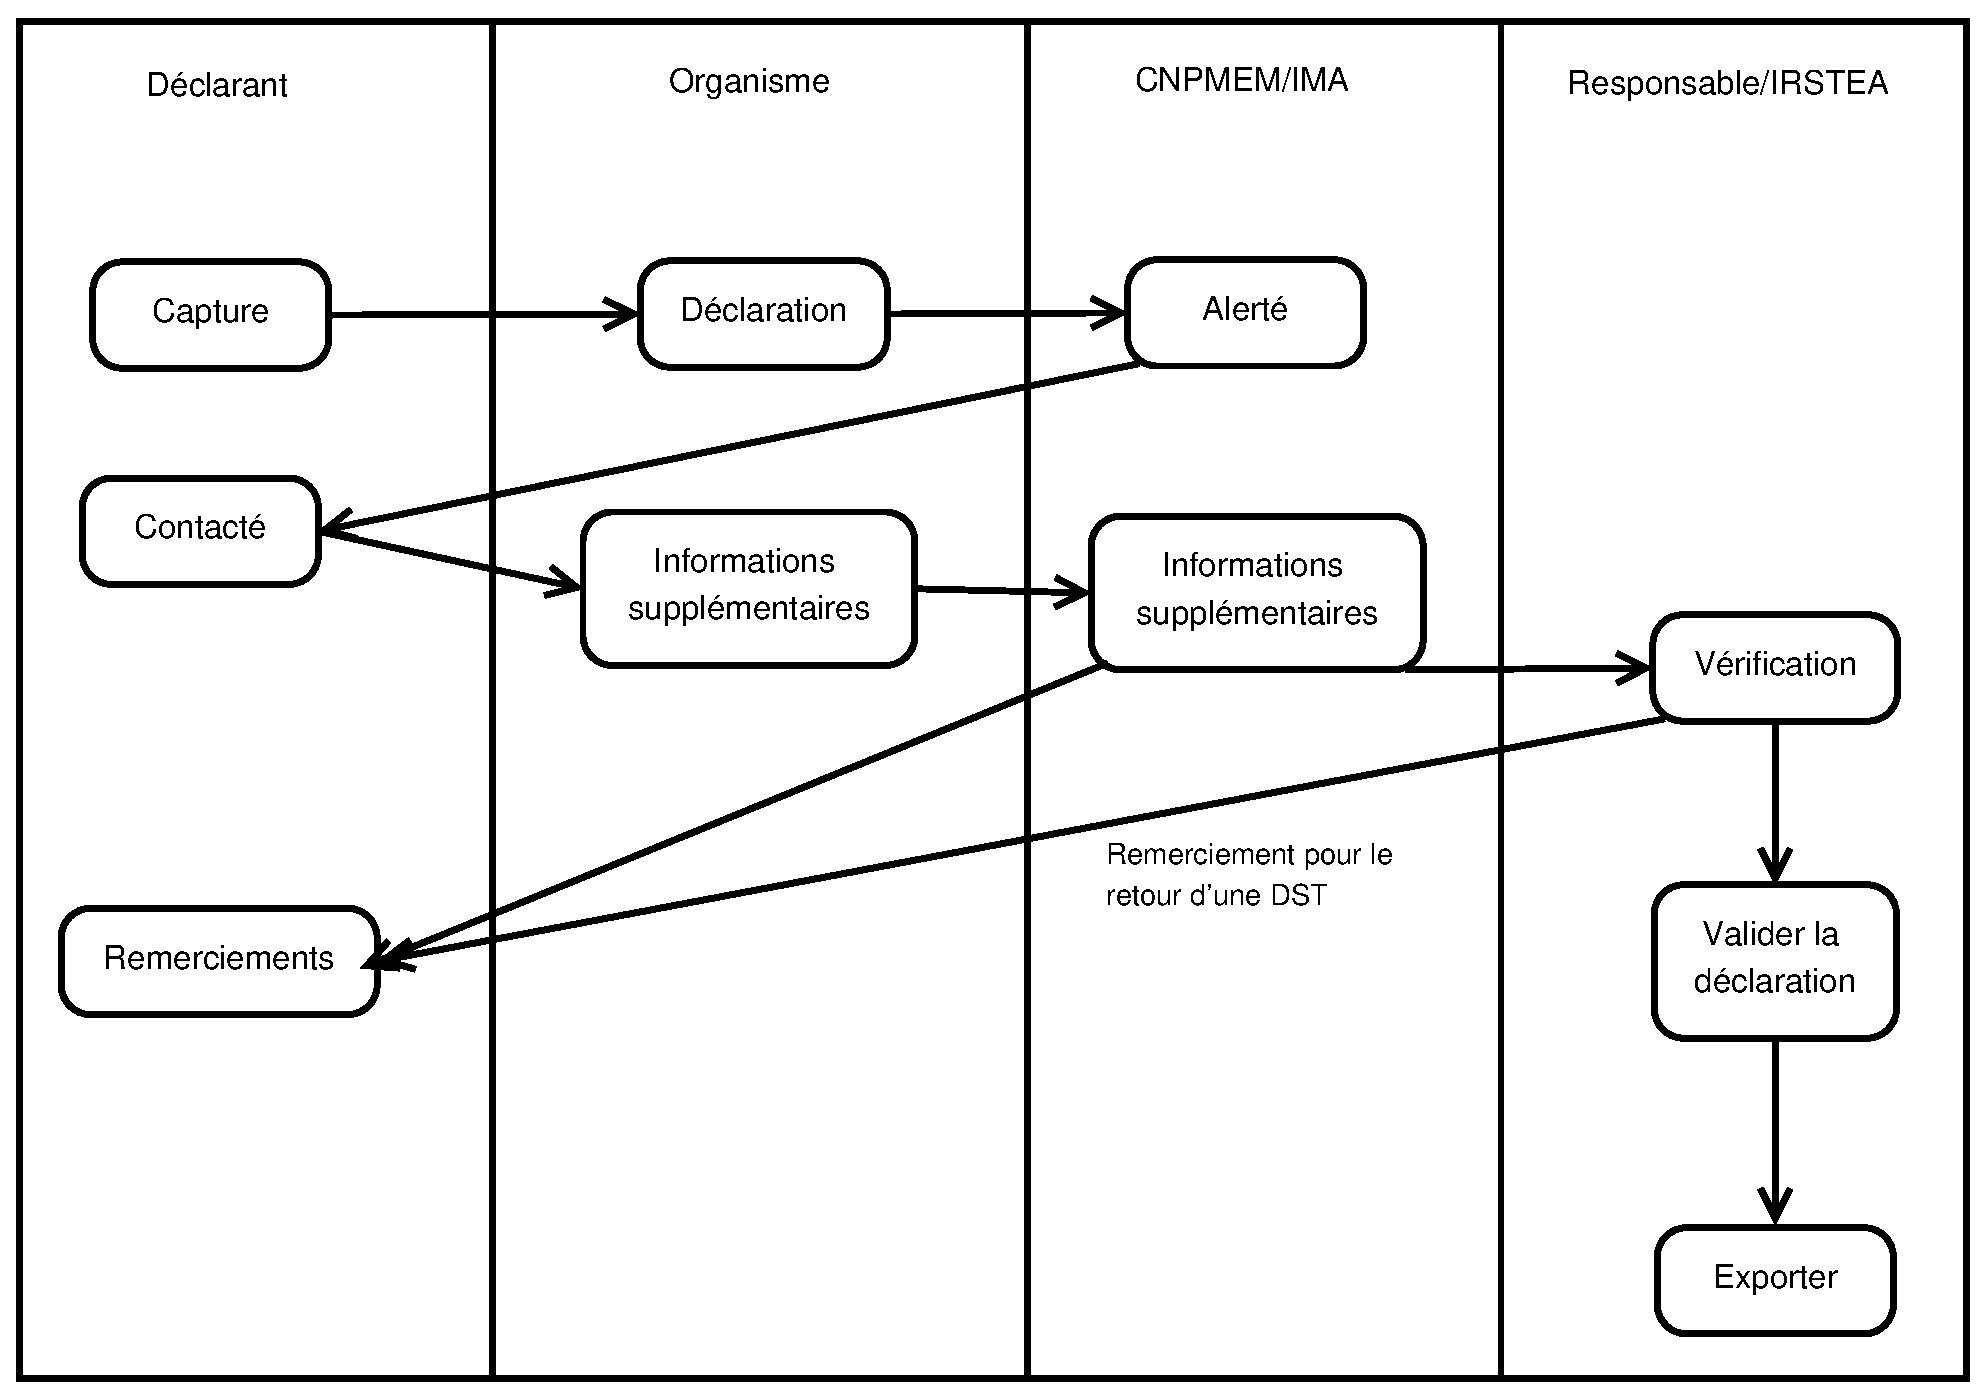
\includegraphics[width=\textwidth]{pictures/schemaDeclaration.eps}
\caption{Menu principal}
\end{figure}

Le pêcheur, qu'il soit amateur ou professionnel, se doit de déclarer la prise d'un esturgeon. Les informations récoltées  lors de la déclaration peuvent être recueillies par différents organismes tels que le CNPMEM (\textit{Comité National des Pêches Maritimes et des  Marins}), l'IMA (\textit{l'Institut des Milieux Aquatiques}) ou Irstea. Une fois les déclarations saisies, elles sont transmises à Irstea. Après une phase de contrôle et de vérification effectuée par le responsable du projet, l'ensemble des informations obtenues sont traitées puis partagées avec tous les partenaires du PNA: l'IMA, le CNPMEM, Migado et la DREAL.

J'ai reçu une copie du fichier Excell où se trouvent toutes les données déjà enregistrées à transformé en base de données.

\section{Création de la base de données}
Les informations renseignées par le responsable du projet se répartissaient dans 48 colonnes suivant un ordre précis pour les rentrer rapidement. Il fallait que je transforme le tableur en base de données facilement exploitable aussi bien par une application Web que par des scientifiques. Grâce au logiciel Power Architect, j'ai déjà créé le schéma de structure de la base afin d'avoir une vue d'ensemble et de définir les différentes tables avec les bons attributs. Une fois le schéma créé, et plusieurs réunions pour vérifier la justesse de celui-ci, le logiciel m'a permis d'exporter un script SQL. Pour utiliser ce script, il faut le copier et le lancer avec SQL Workbench. 

Tout au long du stage et du développement, j'ai modifié la base de façon régulière pour me permettre d'obtenir ce que je voulais et de corriger les erreurs qui étaient passées lors de la création.

\section{Application Web}
\subsection{Code et explications de code}
Dans le framework prototypePHP, Smarty est un moteur de template qui permet de séparer la partie applicative de la partie apparence, interface. Grâce à cela, on améliore la lisibilité du code et on se retrouve avec un code simple, facile d'apprentissage. L'affichage sera géré en quatre étapes : 
\begin{itemize}
\item Demande d'exécution du script PHP par le navigateur;
\item Différents modules de l'application sont appelés par le script pour traiter ce qui est demandé. C'est ici que les classes vont être instanciés, les informations issues de la base de données vont être traitées;
\item A chaque fois que le script voudra envoyer des informations, il fera appel au bon module qui se chargera de l'affichage;
\item Une fois le script terminé, le module d'affichage enverra le gabarit et affichera la page HTML au navigateur.\newline
\end{itemize}

	Le code de l'annexe 1 représente une partie du switch qui permet à Smarty d'utiliser le bon template suivant le choix de l'utilisateur. Par soucis de praticité, ne figure que la partie liste.
Une fois que le paramètre a été identifié comme étant "list" (voir paragraphe suivant), on va attribuer à différentes variables les paramètres de la requête HTML. Si l'utilisateur a effectué une recherche, le paramètre \textit{isSearch} va passer à vrai et va permettre d'entrer dans le \textit{if}. Dans cette structure, on va assigner à la variable \textit{data} le résultat d'une requête SQL créée dans la classe Capture qui retourne les enregistrement qui correspondent au(x) critère(s) de recherche. Puis Smarty se chargera d'envoyer la page HTML avec les bonnes données issues du résultat de cette requête. 
Sinon, Smarty affichera toutes les données de la table concernée.\newline\newline
\clearpage
La liste des paramètres qu'utilise le switch se trouve dans un fichier XML consulté par Smarty (voir annexe 2). 
\newline

\textbf{action} permet d'indiquer à Smarty où envoyer le paramètre, qui se trouve dans \textbf{param}. \textbf{menulevel} définit la place de l'action par rapport à la barre de menu, sur le même principe, \textbf{menuorder} représente l'ordre de l'action par rapport au \textbf{menulevel}. Evidemment, \textbf{menudroits} gère les droits de l'utilisateur qui a émis la requête. Enfin, l'intitulé de l'action sera la valeur ou le texte entré dans \textbf{menuvalue}. Ici, la valeur 44 de menuvalue est stockée dans un fichier qui ne contient que des messages attribués à des valeurs. 44 affiche "Capture". Par conséquent, une action "Capture" visible tout de suite dans le menu principal (si la valeur de menulevel avait été 1, "Capture" serait un sous menu), placé en dixième position. Tous les utilisateurs ont accès à cette action vu que les droits sont vides. On obtient cet affichage :\newline

\begin{figure}[h]
\centering
\includegraphics[scale=0.5]{pictures/menuprincipal.png}
\caption{Menu principal}
\end{figure}
(L'utilisateur ne s'étant pas connecté, toutes les options de ce menu n'apparaissent pas et "Capture" ne se retrouve pas réellement en dixième position.)

Le template utilisé par Smarty est un fichier \textit{.tpl} qui contient uniquement du HTML. Smarty nous permet d'utiliser des fonctions que l'on ne trouve pas en HTML telles que le \textit{if} qui permet les tests, le \textit{section} qui permet les boucles et le \textit{strip} qui permet d'écrire sur plusieurs lignes. 
Le code de l'annexe 3, simplifié, est le template qui permet d'afficher la liste des captures. On peut voir trois fonctions différentes de Smarty. La première est la fonction \textit{include}. Ici, elle permet d'inclure et d'afficher le gabarit en charge des critères de recherche (et qui permet de modifier la valeur de \textit{isSearch}). On trouve aussi la fonction \textit{if} qui permet de tester une variable et d'afficher en conséquence. Enfin, la fonction \textit{section} qui permet de boucler sur la variable \textit{data} et d'afficher les données pour chaque enregistrement.
\clearpage
\subsection{Paramètres}
Pour faciliter un maximum l'utilisation de l'application, l'utilisateur à la possibilité de créer des paramètre utilisable dans le formulaire de déclaration principal. Cette fonctionnalité se trouve dans le menu principal, dans la section "Paramètres".  Les paramètres sont préalablement définis dans la base de données et sont stockés dans des tables de paramètres.

\begin{figure}[h]
\centering
\includegraphics[scale=0.8]{pictures/menuParam.png}
\caption{Menu et sous-menu des paramètres}
\end{figure}

Une fois que l'utilisateur à cliqué sur le paramètre voulu, il est redirigé vers la liste des paramètres. Celle-ci contient le libellé au minimum. Mais pour le cas des engins (figure 3.3), on a le libellé, le type et le maillage. Chaque paramètre doit être unique, il pourra être réutilisé plus tard autant de fois que le souhaite l'utilisateur.\newline

\begin{figure}[h]
\centering
\includegraphics[scale={0.8}]{pictures/paramList.png}
\caption{Liste des informations du paramètre "Engin"}
\end{figure}
\clearpage
Devant cette liste, deux choix s'offrent à l'utilisateur : Créer un nouveau paramètre en cliquant sur "Nouveau", modifier un paramètre déjà existant en cliquant sur l'un des libellé de la liste.
Dans le premier cas, le navigateur affiche un formulaire vierge de saisie de paramètre. L'affichage est basique mais très simple à comprendre. On renseigne le(s) champ(s) souhaité(s), et on enregistre la saisie. Le formulaire de modification repose sur le même principe, la seule différence réside dans le fait que le(s) champ(s) sont en partie ou intégralement renseigné.\newline

Cette méthode de création de paramètre s'applique pour les informations en lien avec la localisation (région, pays, milieu, zones ciem), les espèces et les engins. Une fois que le chercheur a créé tout les paramètres dont il aura besoin, il peut également consulté la liste des individus capturés dont la déclaration a déjà été enregistrée. 

\begin{figure}[h]
\centering
\includegraphics[width=\textwidth]{pictures/paramModif.png}
\caption{Formulaire de modification de paramètre}
\end{figure}

\begin{figure}[h]
\centering
\includegraphics[width=\textwidth]{pictures/paramNouveau.png}
\caption{Formulaire de création de paramètre}
\end{figure}
\clearpage

\subsection{Liste, détails et modification d'une capture}
En cliquant sur l'onglet "Capture", un encadré de recherche permet d'afficher des captures selon des critère précis. Si aucun de ces champs n'est rempli, tous les enregistrements de la base sont affichés. Les intitulés des colonnes ont été choisi de façon à rendre la recherche la plus pertinente possible, tout en gardant l'ordre initial des colonnes du fichier Excel.
Ici aussi, les paramètres sont exploités et on retrouvera ceux enregistré, suivant la méthode énoncée plus haut, dans les listes déroulantes. Grâce à du JQuery, un calendrier apparaît sous les zones de saisie associées aux dates. 

\begin{figure}[h]
\centering
\includegraphics[width=\textwidth]{pictures/listeCapture.png}
\caption{Liste et encadré de recherche}
\end{figure}

Quelques fonctions d'exportation existent (PDF, CSV, impression simple par navigateur). Cependant, même si les deux dernières fonctionnent, l'export en PDF n'est pas adapté et l'affichage n'est pas idéal.
L'utilisateur peut ajouter autant d'entrées qu'il le souhaite, une navigation facile permet de charger des pages avec un certain nombre d'entrées puis de les parcourir grâce aux flèches en-dessous de la liste.

\clearpage
Pour créer une nouvelle capture, un formulaire vierge apparaîtra après que l'utilisateur ai cliqué sur "Nouveau". On retrouve le même principe qu'avec les paramètres. L'intégralité des informations de chaque capture n'est pas affiché ici. C'est en cliquant sur l'icône de feuilles que l'utilisateur aura accès aux détails associés à la capture correspondante. Sur cet écran (figure 3.7), y figure les données des engins, les individus associés, les évènements et les remerciements que le responsable pourra ajouter au fur et à mesure, etc. On remarquera que ces derniers éléments cités sont différents des autres renseignements. En effet, ils ont les mêmes propriétés que la liste vu plus haut. L'utilisateur à la possibilité de modifier n'importe quelle capture en cliquant sur le lien "Modifier". Pour retourner à la liste des individus capturés, l'utilisateur devra cliquer sur "Retour à la liste". 

\begin{figure}[h]
\centering
\includegraphics[width=\textwidth]{pictures/detailCapture.png}
\caption{Liste et encadré de recherche}
\end{figure}
\clearpage

Tout les champs peuvent être modifiés et seront enregistrés lorsqu'on pressera le bouton d'enregistrement. Chaque information est récupérée suivant la capture dont est issue la page de modification puis inséré dans la bonne zone de texte.
\begin{figure}[h]
\centering
\includegraphics[width=\textwidth]{pictures/modifCapture.png}
\caption{Fragment du formulaire de modification de capture}
\end{figure}\newline
Le formulaire de création de capture est identique à celui-ci. Cependant, aucune information n'est affichée car aucune n'est associée. 
\clearpage
Lorsque l'utilisateur veut ajouter un individu, un évènement ou un remerciement à sa déclaration, il lui suffit de cliquer sur le lien "Nouveau" associé au bon module. Il sera redirigé vers un formulaire vierge pour le remplir. Il sera automatiquement associé à la bonne capture.
Si l'utilisateur veut modifier une de ces , on retrouve le même principe énoncé plus haut, on accède à un formulaire de modification de l'individu, de remerciements ou d'évènement. 

\begin{figure}[h]
\centering
\includegraphics[width=\textwidth]{pictures/modifIndividu.png}
\caption{Fragment du formulaire de modification d'individu}
\end{figure}

\section{Fonctionnalités complémentaires}

Aux terme du stage, l'application est entièrement fonctionnelle et peut être utilisée tel quel. Cependant, quelques fonctions n'ont pas été implémenté mais n'empêche pas l'utilisation du projet.

Afin que les acteurs du projet sturwild soient tous avertis, on pourra implémenter une fonction de messagerie ou d'envoi de messages automatique ainsi qu'un suivis de ces message sur le même principe que les remerciements et évènements. 

De plus, l'exportation PDF pourra être amélioré et sera consultable par les utilisateurs. Ce document fera office de base de données visible et officiel auprès de l'IMA, Irstea et du CNPMEM.

Enfin, on pourra gérer les droits d'accès aux utilisateurs, cette gestion se faisant facilement grâce au module phpGacl de protoypePhp. Certains login seront associé à la consultation et la modification tandis que d'autre seront juste autorisé à consulter. 
\clearpage
\LARGE{Conclusion}\normalsize\newline

Durant ce stage, j'ai développé un projet qui s'est montré complet aussi bien durant la conception que durant le développement : l'application de suivi des captures accidentelles d'esturgeons a pour but d'aider à la prise de déclaration, au transfert de données et à la communication entre les acteurs. L'application devait être opérationnelle pour la fin du stage, début juin.

Pour réaliser ce projet, j'ai dû adopter un aspect multitâche : je devais préparer la conception, créer et gérer la base de données et développé une application web. Lors de la phase conceptuelle, je devais sortir de l'aspect technique habituel et plus me concentrer sur l'aspect utilisateur. L'intégralité de mes notes devait être comprise d'une personne lambda. Par conséquent, j'ai du être le plus rigoureux possible tout en tenant compte des termes et des tournures de phrases employés dans le rapport des cas d'utilisation. Ensuite, la base que j'ai créé va être utilisée dans le futur, avec sans doute quelques modifications. Elle doit donc être correcte et là aussi facilement compréhensible. Enfin, même si mon application ne contient pas les fonctionnalités complémentaires, elle fonctionne parfaitement et peut être utilisée.\newline

L'utilisation des méthodes agiles m'a permis d'avoir un dialogue régulier avec mon maître de stage, ce qui m'a permis d'avoir un fil directeur tout au long du stage.

   	
\chapter{Annexes}
\section{Annexe 1}
\lstset{language=PHP}
\begin{lstlisting}[frame=single]
switch ($t_module ["param"]) {
	case "list":
		$searchCapture->setParam ( $_REQUEST );
		$dataSearch = $searchCapture->getParam ();

		if ($searchCapture->isSearch () == 1) {
			$_SESSION ["searchCapture"] = $searchCapture;
			$data = $dataClass->getListeSearch ( $dataSearch );			
			$smarty->assign ( "data", $data );
			$smarty->assign ( "isSearch", 1 );
		}
		$smarty->assign ( "captureSearch", $dataSearch );
		$smarty->assign ( "corps", "capture/captureList.tpl" );
		break;
}
\end{lstlisting}
\section{Annexe 2}
\lstset{language=XML}
\begin{lstlisting}[frame=single]
<captureList action="modules/capture/capture.php" param="list" menulevel="0" menuorder="10" menudroits="" menuvalue="44" />
\end{lstlisting}
\section{Annexe 3}
\lstset{language=HTML}
\begin{lstlisting}[frame=single]
{include file="capture/captureSearch.tpl"} {if $isSearch == 1}
 <a href="index.php?module=captureChange&id=0" class="left"> Nouveau</a> <br>
<script>
	setDataTables("captureListe");
</script>
<table id="captureListe" class="tableliste">
	<thead>
		<tr>
			<th> Acces aux captures</th>
			<th>Espece</th>
			<th>Masse <br>(en Kg)</th>
			<th>Longueur<br>(en mm)</th>
			<th>Engin</th>
		</tr>
	</thead>
	<tdata> {section name=lst loop=$data}
	<tr>
		<td><a href="index.php?module=captureDisplay&id={$data[lst].capture_id}"><img src="display/images/declaration.png"></a>
		<td>{$data[lst].espece}</td>
		<td>{$data[lst].poids}</td>
		<td>{$data[lst].longueur_individu}</td>
		<td>{$data[lst].engin}</td>
	</tr>
	{/section} </tdata>
</table>
{/if}
\end{lstlisting}
\end{document}
